\section{Realisation et mise en oeuvre}
\subsection{Sprint 1: D´eveloppement et D´eploiement du Chatbot}
\begin{frame}{Diagramme de cas d'utilisation}

    \begin{figure}[H]
        \centering
        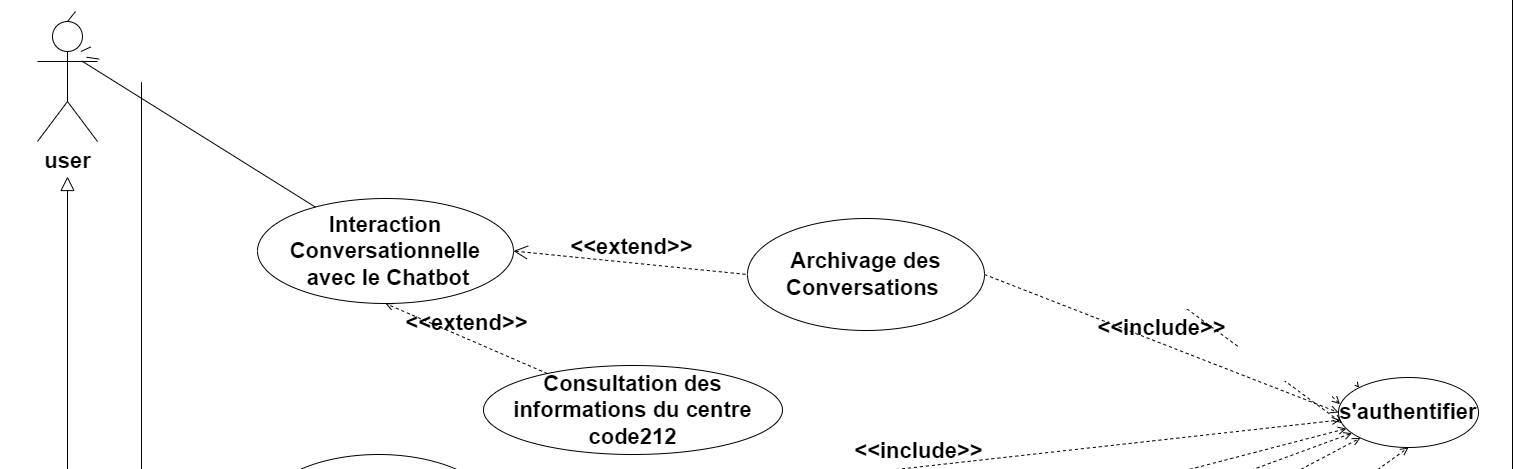
\includegraphics[height=4cm]{assets/images/sprint1-usecase.png}
    \end{figure}
\end{frame}

\begin{frame}{Diagramme de classe}

    \begin{figure}[H]
        \centering
        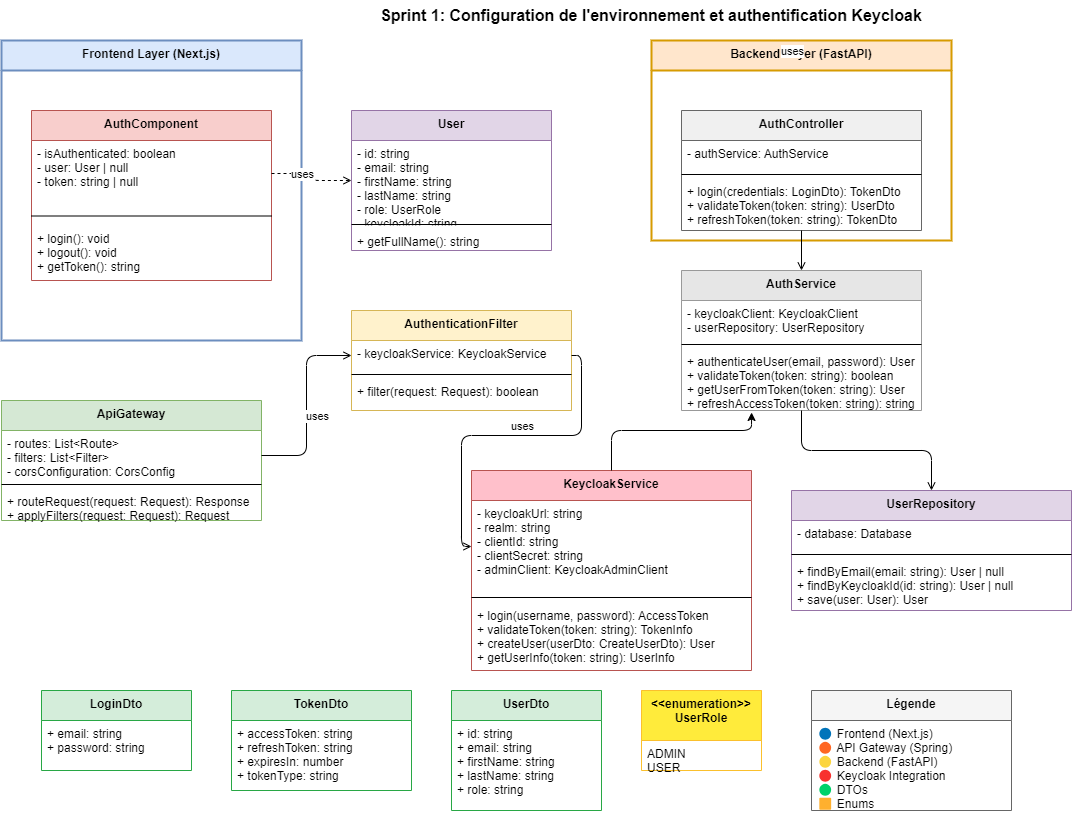
\includegraphics[height=5cm]{assets/images/sprint1-class.png}
    \end{figure}
\end{frame}

\begin{frame}{Diagramme de sequence}
    \begin{figure}[H]
        \centering
        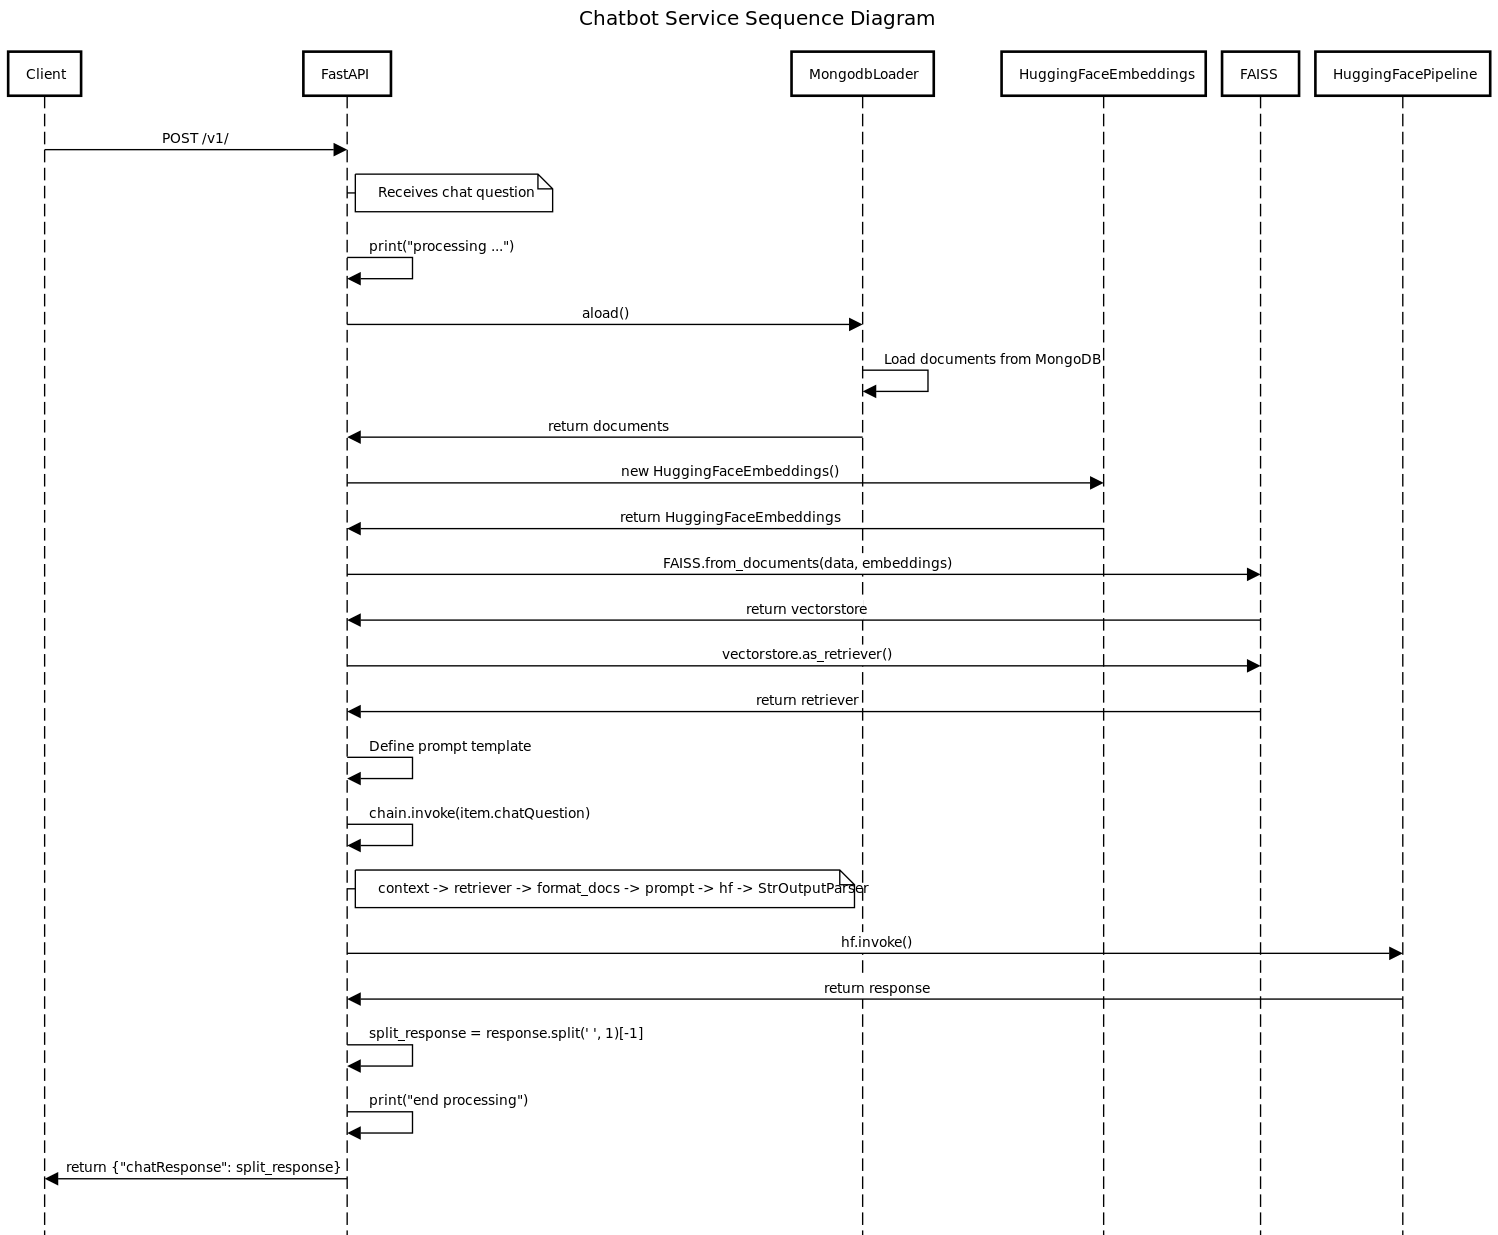
\includegraphics[height=8cm]{assets/images/chatbot-seq.png}
    \end{figure}
\end{frame}

\begin{frame}{Realisation}
    \begin{figure}[H]
        \centering
        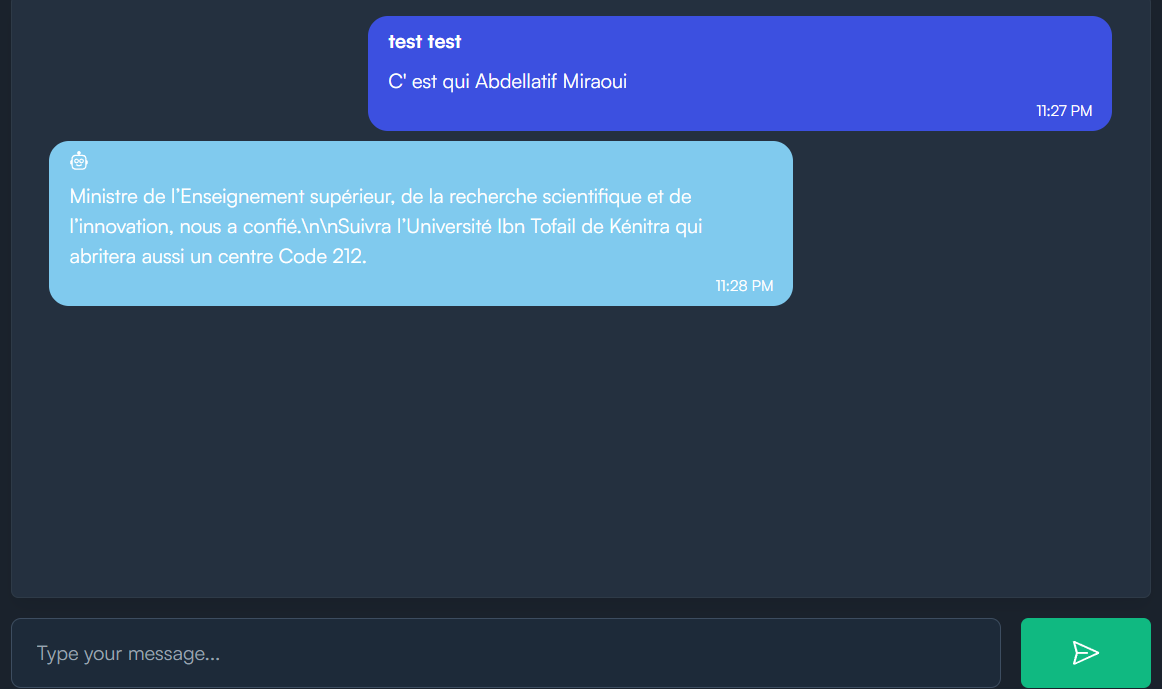
\includegraphics[height=6cm]{assets/images/chat2.png}
    \end{figure}
\end{frame}


\subsection{Sprint 2: Authentification et mise a jour de la
    base de donnees par l’administrateur}
\begin{frame}{Diagramme de cas d'utilisation}

    \begin{figure}[H]
        \centering
        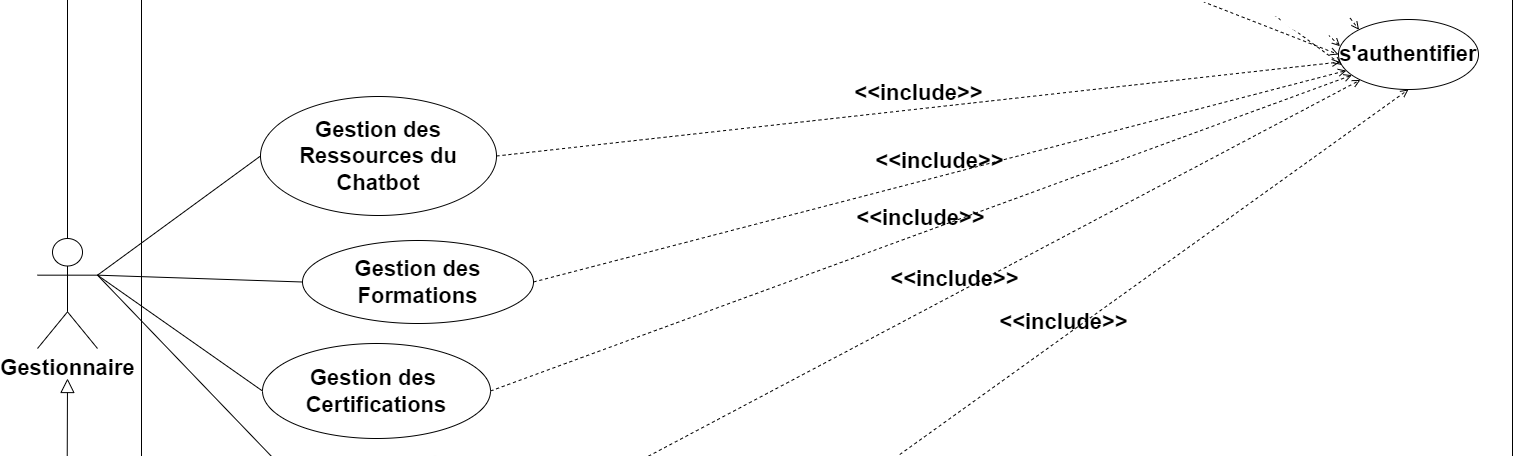
\includegraphics[height=4cm]{assets/images/sprint2-usecase.png}
    \end{figure}
\end{frame}

\begin{frame}{Diagramme de classe}

    \begin{figure}[H]
        \centering
        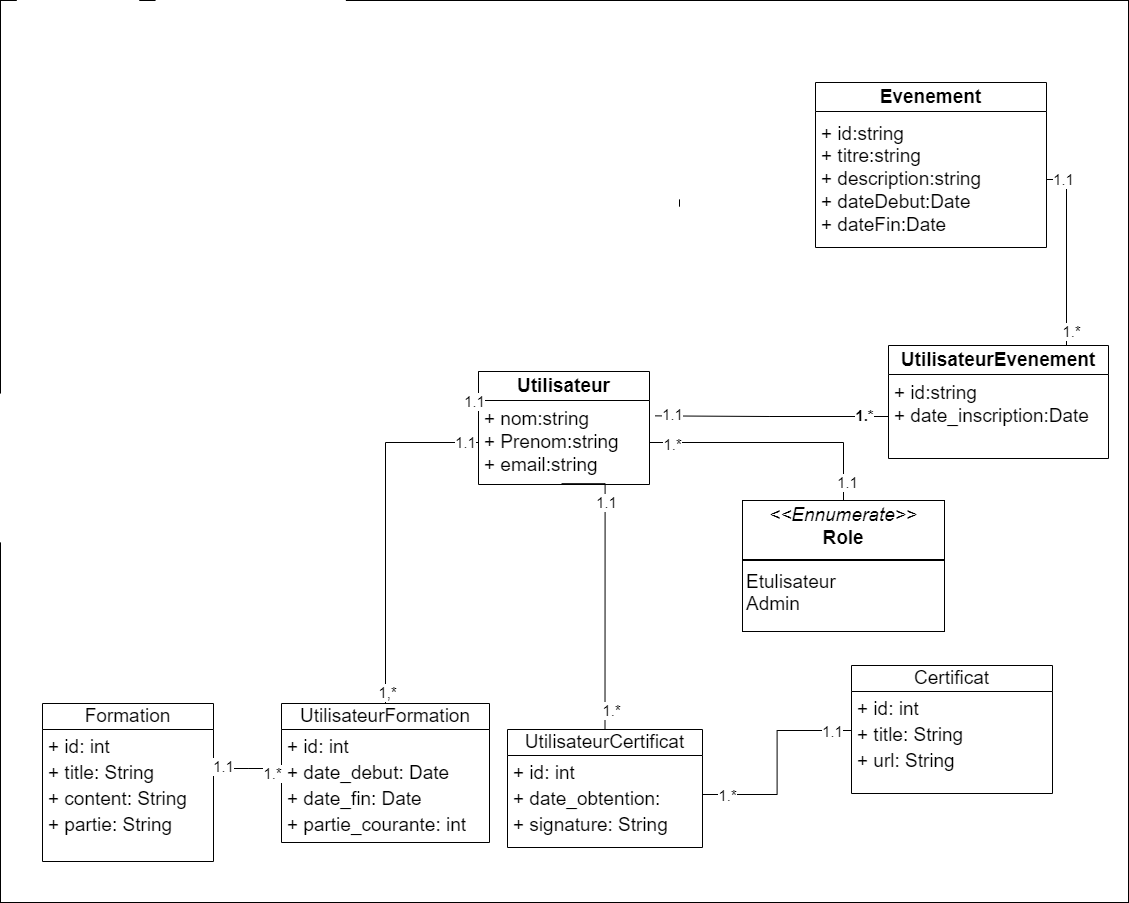
\includegraphics[height=5cm]{assets/images/sprint2-class.png}
    \end{figure}
\end{frame}

\begin{frame}{Diagramme de sequence d'authentification}
    \begin{figure}[H]
        \centering
        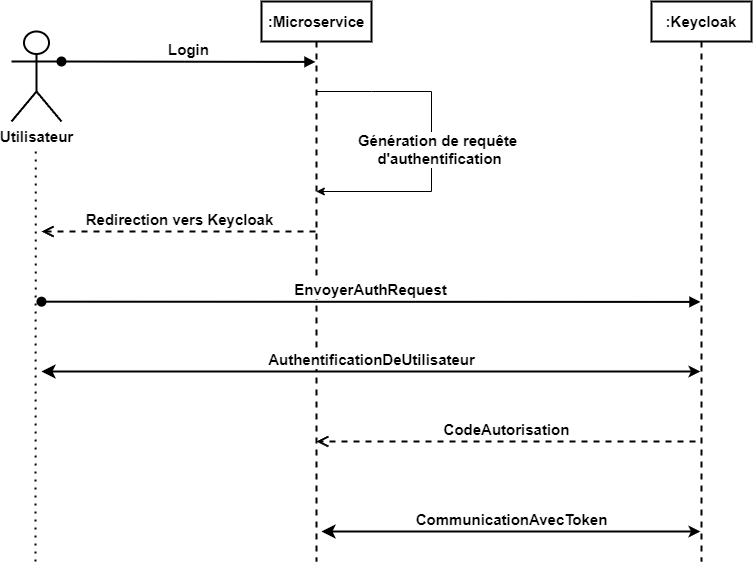
\includegraphics[height=8cm]{assets/images/keycloak-seq.png}
    \end{figure}
\end{frame}

\begin{frame}{Diagramme de sequence de gestion des resources du chatbot}
    \begin{figure}[H]
        \centering
        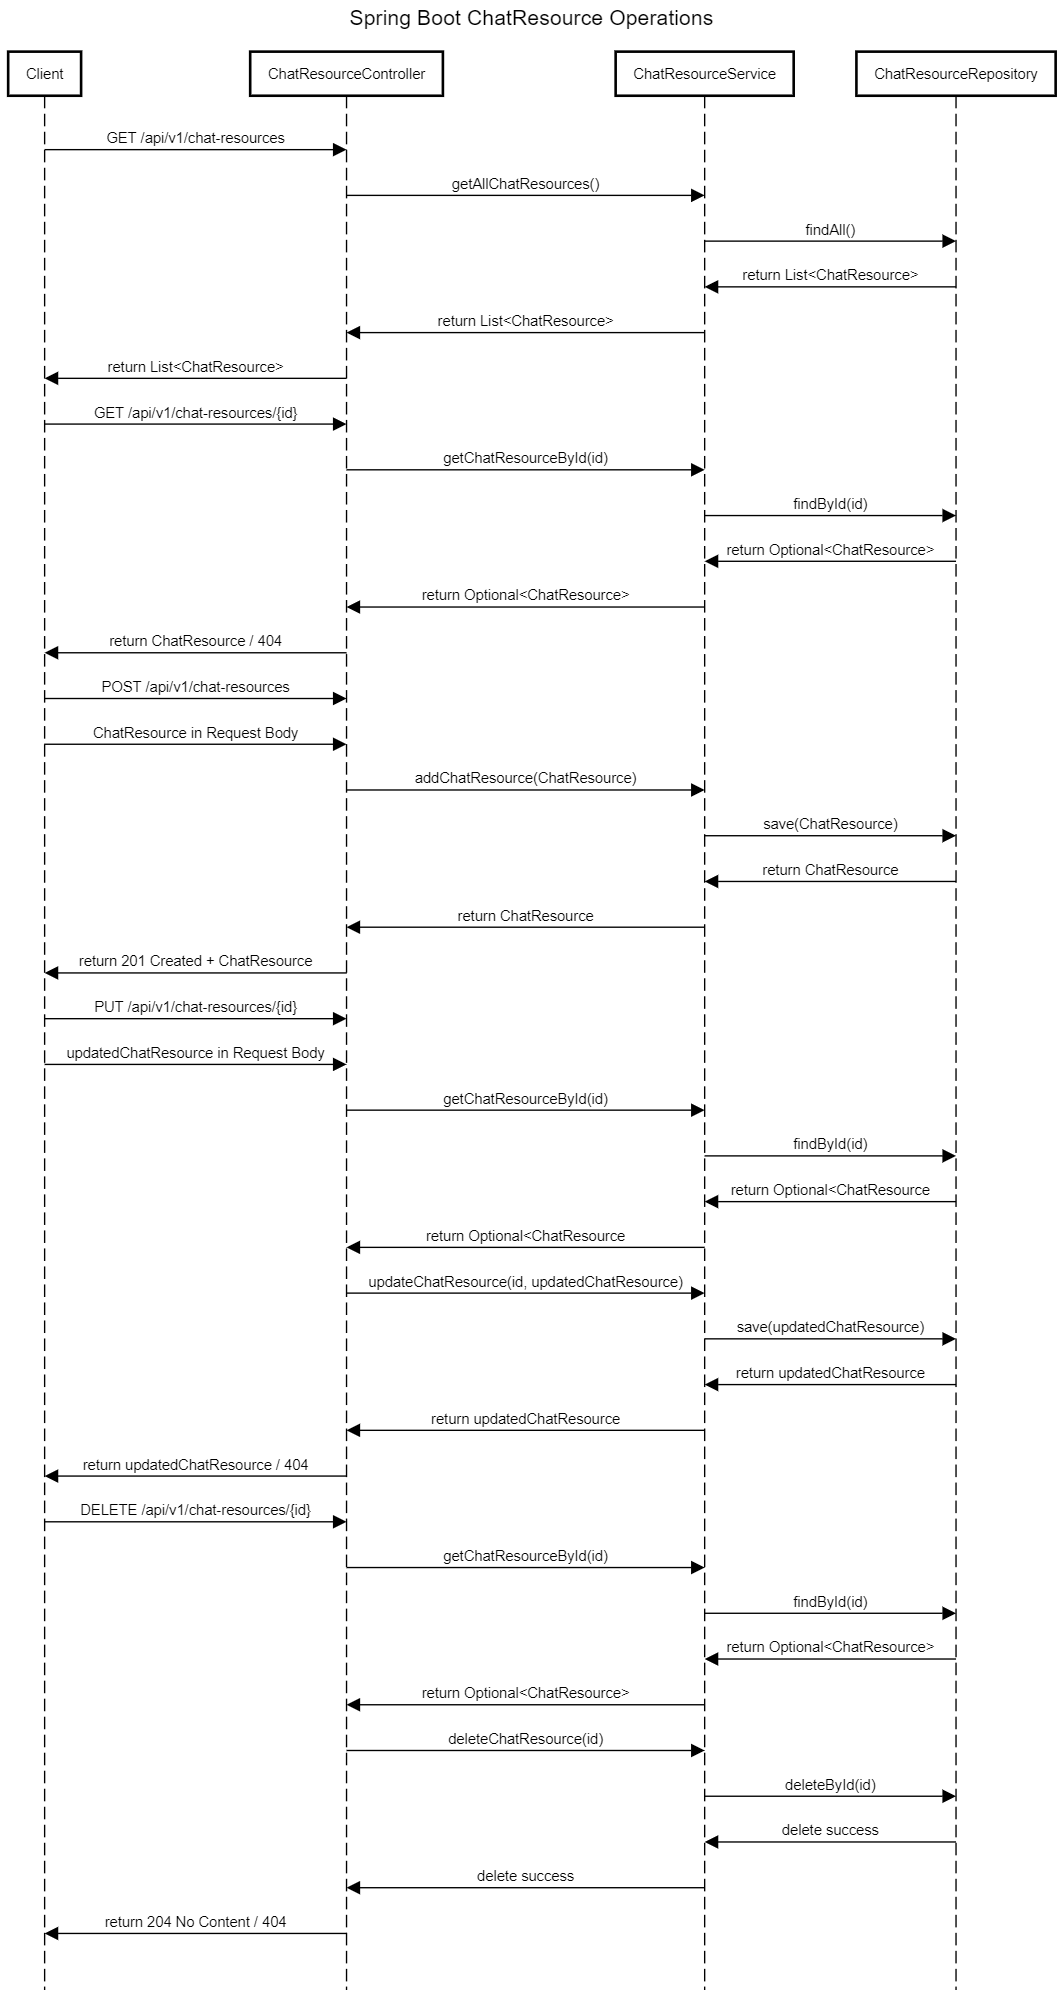
\includegraphics[height=8cm]{assets/images/chat-res-seq.png}
    \end{figure}
\end{frame}

\begin{frame}{Realisation}
    \begin{figure}[H]
        \centering
        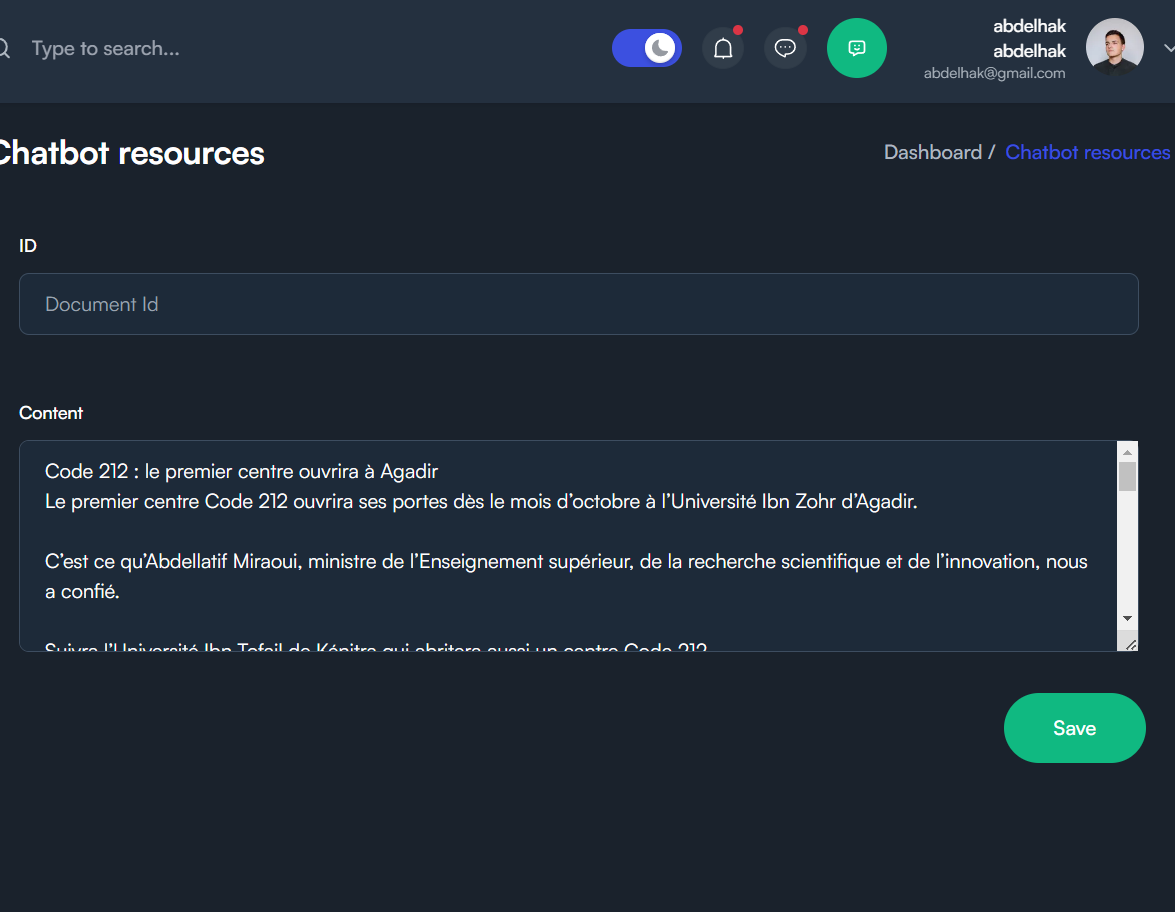
\includegraphics[height=6cm]{assets/images/admin-doc.png}
    \end{figure}
\end{frame}



\subsection{Sprint 3: Inscription aux cours, Eevenements et
    certificats}
\begin{frame}{Diagramme de cas d'utilisation}

    \begin{figure}[H]
        \centering
        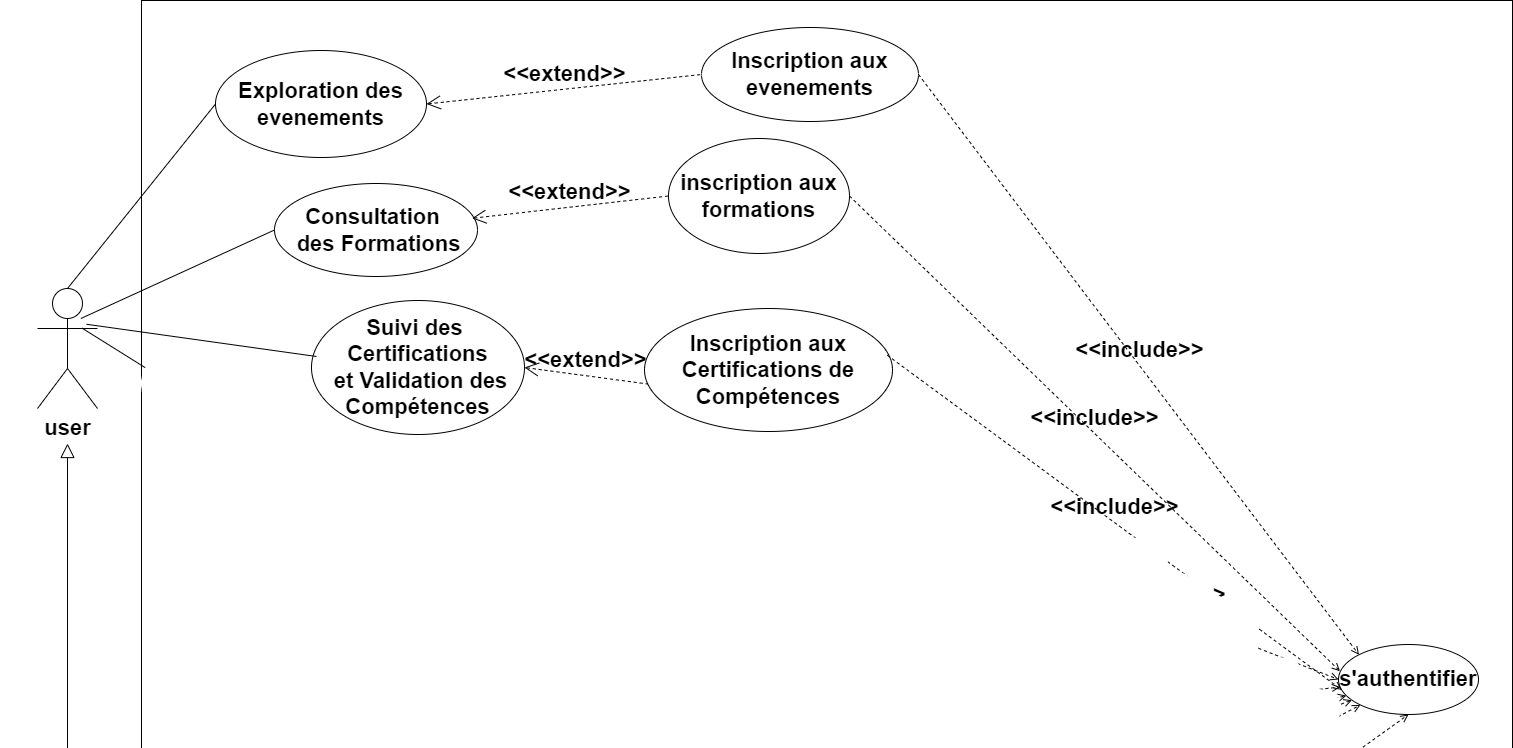
\includegraphics[height=5cm]{assets/images/sprint3-usecase.png}
    \end{figure}
\end{frame}

\begin{frame}{Diagramme de classe}

    \begin{figure}[H]
        \centering
        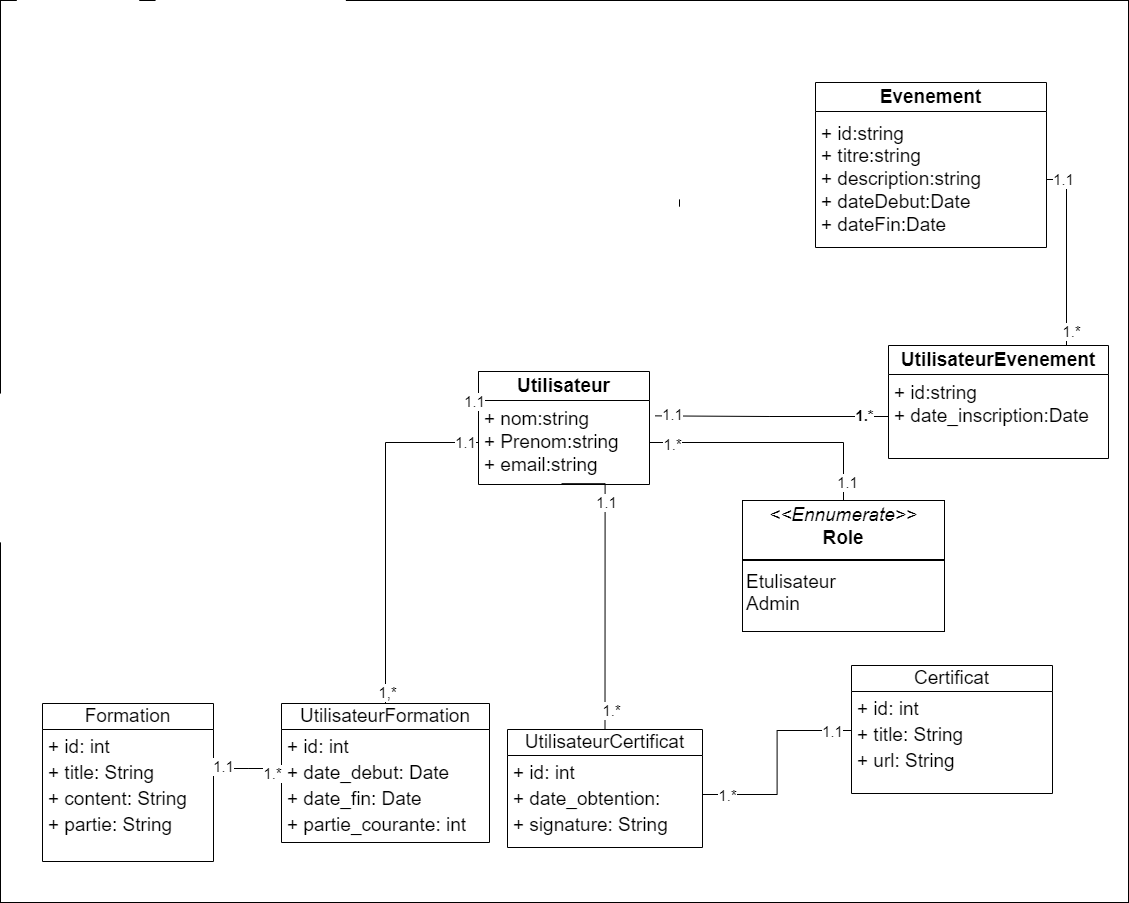
\includegraphics[height=5cm]{assets/images/sprint2-class.png}
    \end{figure}
\end{frame}


\begin{frame}{Diagramme de sequence}
    \begin{figure}[H]
        \centering
        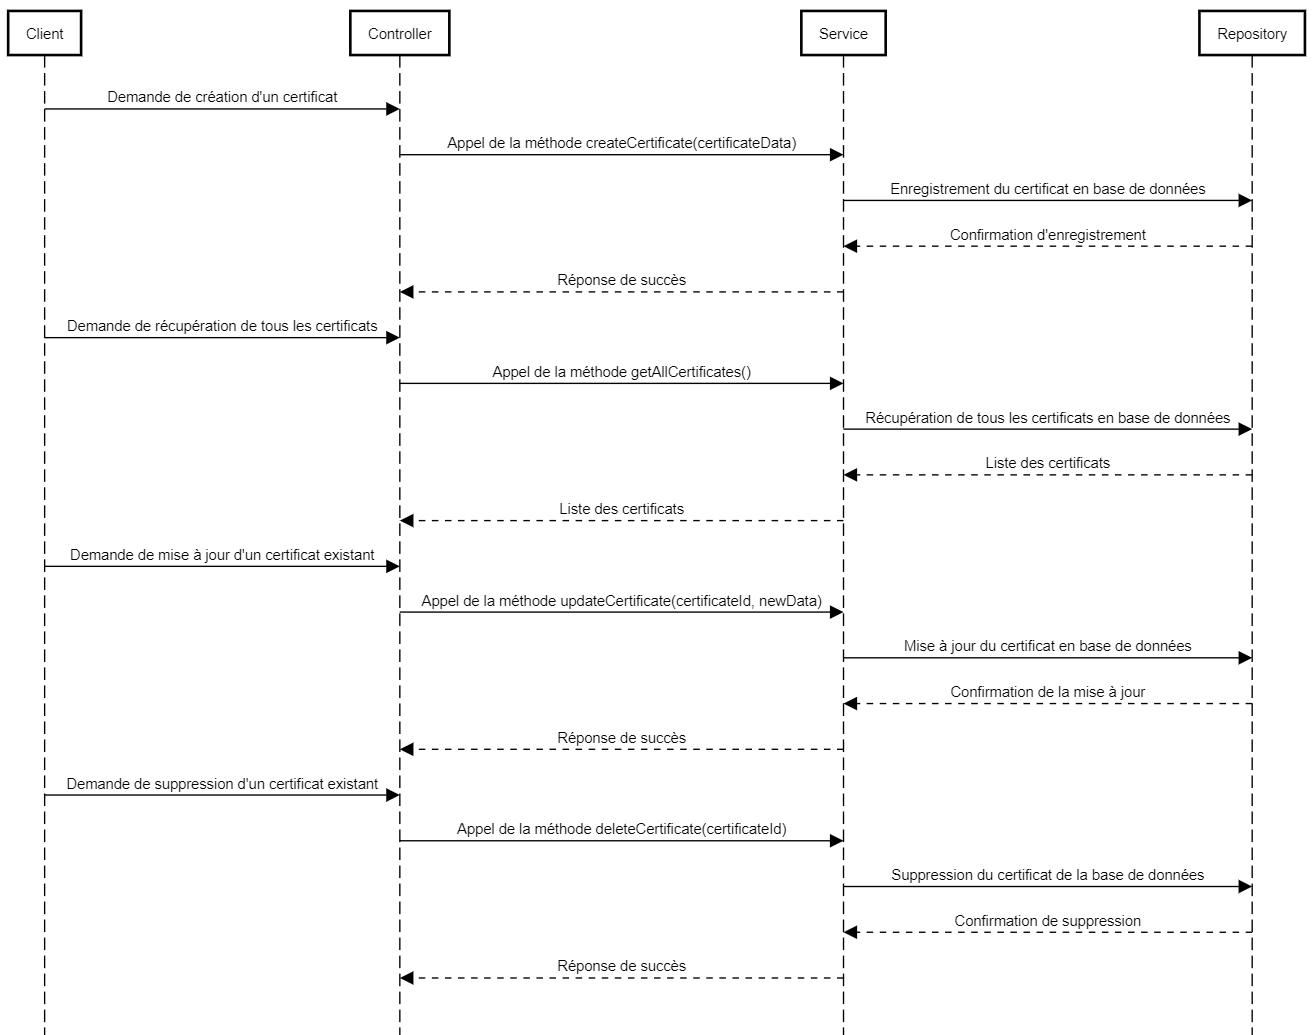
\includegraphics[height=8cm]{assets/images/seq-certifs.png}
    \end{figure}
\end{frame}

\begin{frame}{Realisation}
    \begin{figure}[H]
        \centering
        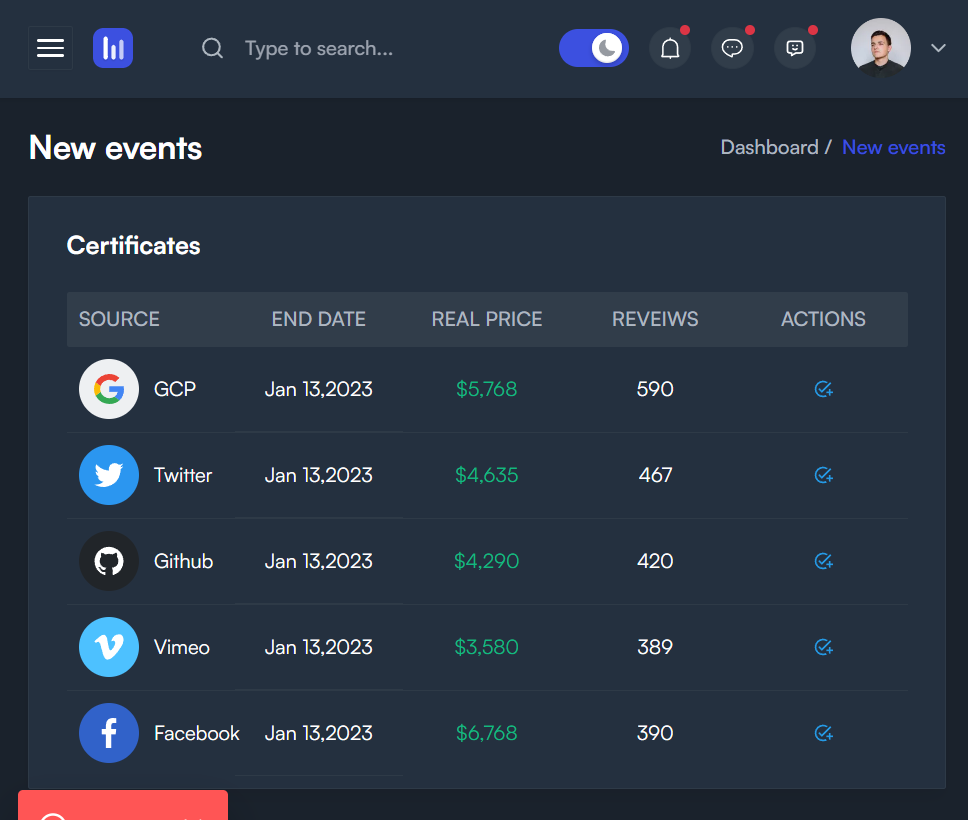
\includegraphics[height=6cm]{assets/images/certifs-list.png}
    \end{figure}
\end{frame}

\begin{frame}{Realisation}
    \begin{figure}[H]
        \centering
        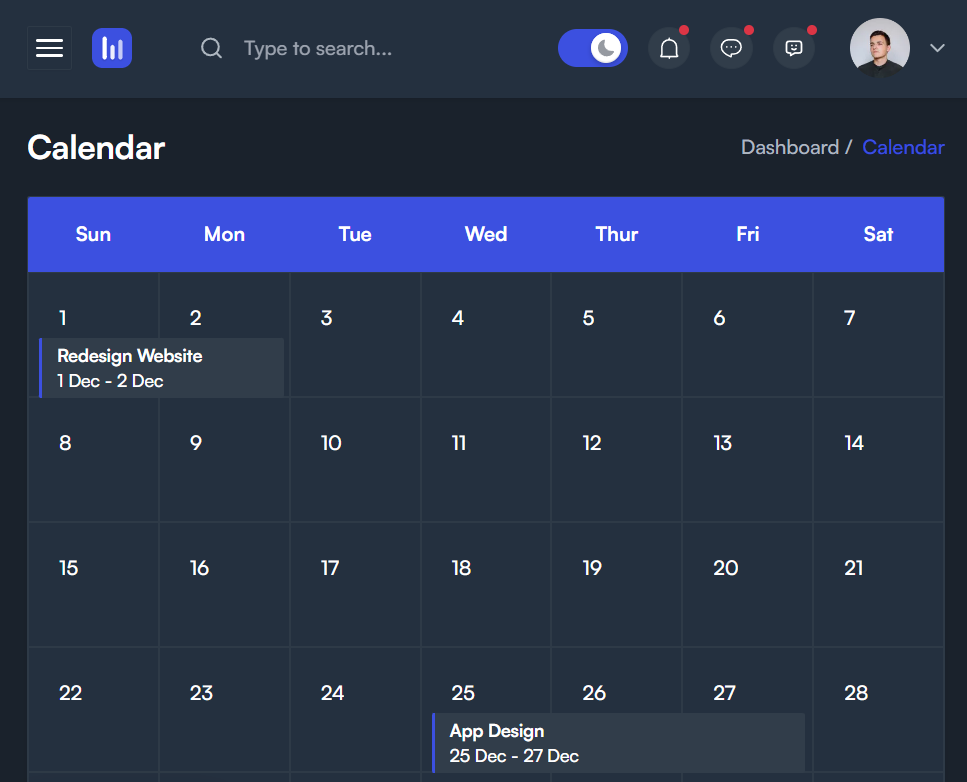
\includegraphics[height=6cm]{assets/images/calendar.png}
    \end{figure}
\end{frame}


\subsection{Sprint 4: Am´elioration de l’Interface Utilisateur et d eploiment et creation des
    contenaires}

\begin{frame}{Chat room en light mode}
    \begin{figure}[H]
        \centering
        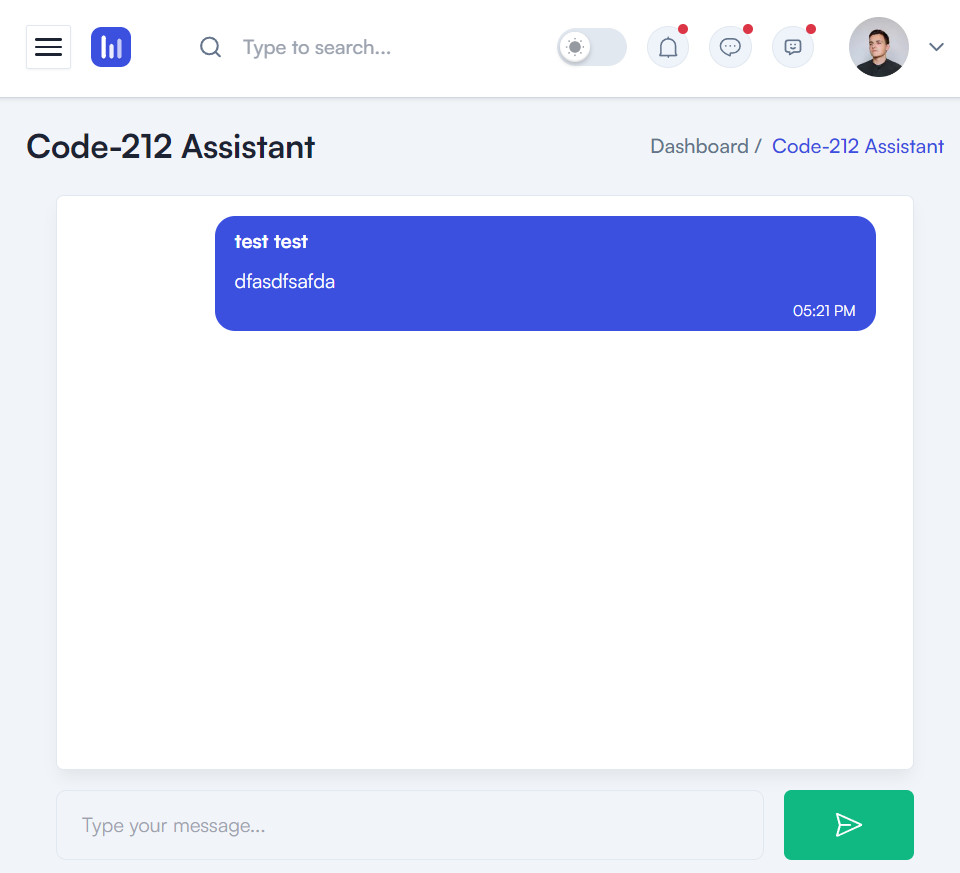
\includegraphics[height=6cm]{assets/images/light-chat.png}
    \end{figure}
\end{frame}

\begin{frame}{Profile en light mode}
    \begin{figure}[H]
        \centering
        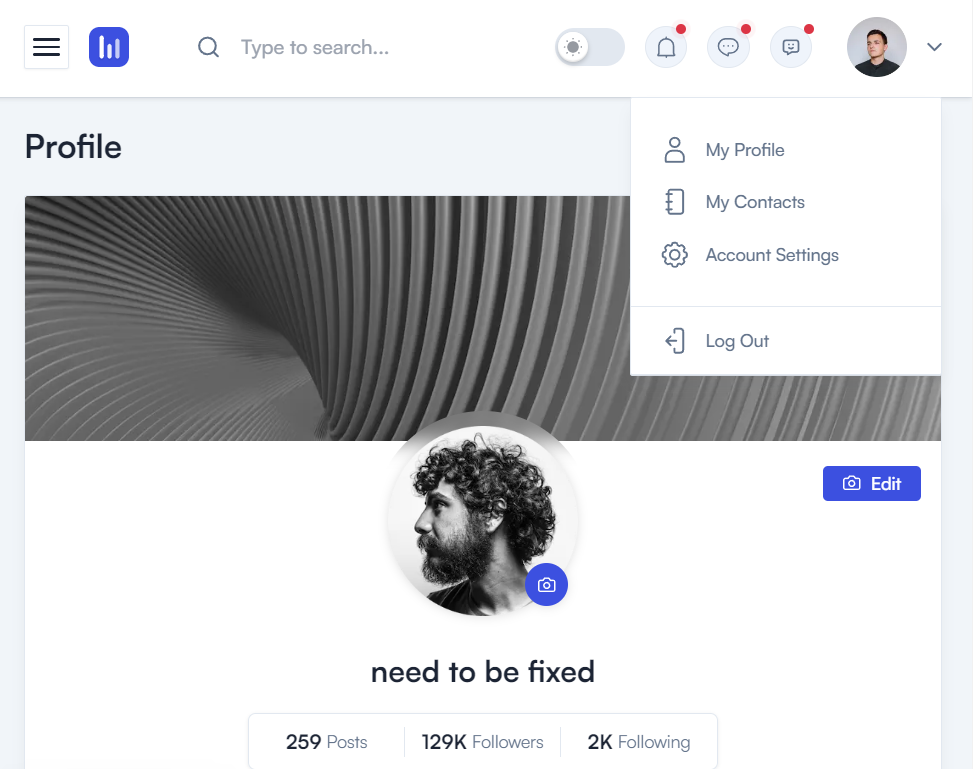
\includegraphics[height=6cm]{assets/images/light-profile.png}
    \end{figure}
\end{frame}

\subsection{Execution}
\begin{frame}{Execution}
    Demonstration de l'application
\end{frame}
